Nu doen we hetzelfde, maar in plaats van equidistante abscissen gebruiken we nu Chebyshev-punten. Het  resultaat voor $sin(x)$ is te vinden in figuur \ref{fig:sincheb}, het resultaat voor $\frac{1}{1+7x^2}$ in figuur \ref{fig:ratcheb}. We geven ook hier steeds een plot van de functiewaarden en van de absolute waarde van het residu weer.

Voor de sinus is er een kleine verbetering ten opzichte van een equidistante verdeling. Voor de andere functie geeft het gebruik van Chebyshev-punten een duidelijke verbetering, vooral aan de rand van het interval. 

Voor de sinus blijft de veelterm een betere benadering dan de splinevoorstelling om dezelfde reden als hierboven vermeld. Voor $\frac{1}{1+7x^2}$ is de veelterm nog steeds een slechtere benadering dan de splinevoorstelling, maar is het verschil tussen beide aan de rand wel kleiner.

\begin{figure}[H]
\centering
\begin{subfigure}{.5\textwidth}
  \centering
  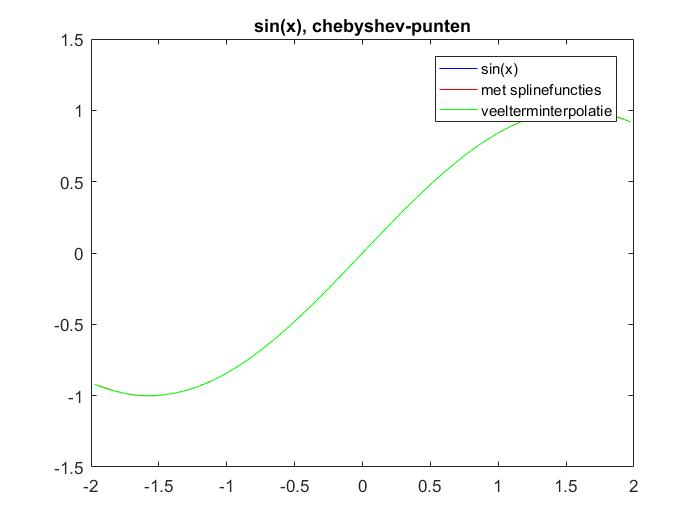
\includegraphics[width=\linewidth]{afbeeldingen/sin_cheb.jpg}
  \caption{functiewaarden}
\end{subfigure}%
\begin{subfigure}{.5\textwidth}
  \centering
  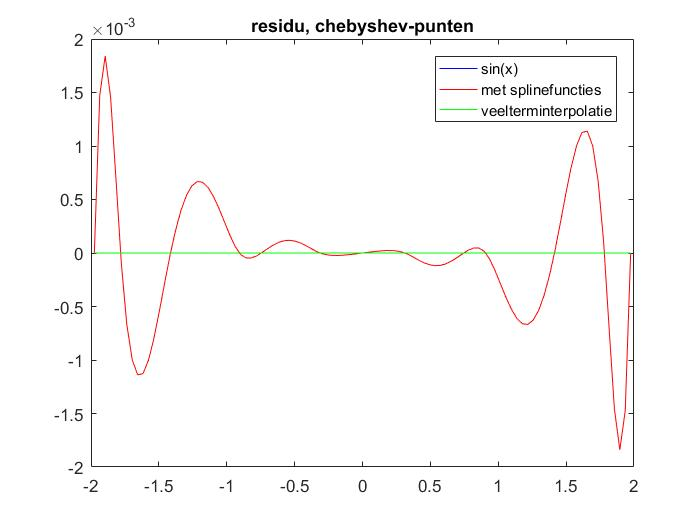
\includegraphics[width=\linewidth]{afbeeldingen/sin_cheb_res.jpg}
  \caption{residu}
\end{subfigure}
\caption{interpolant door 10 Chebyshev-punten van $sin(x)$}
\label{fig:sincheb}
\end{figure}

\begin{figure}[H]
\centering
\begin{subfigure}{.5\textwidth}
  \centering
  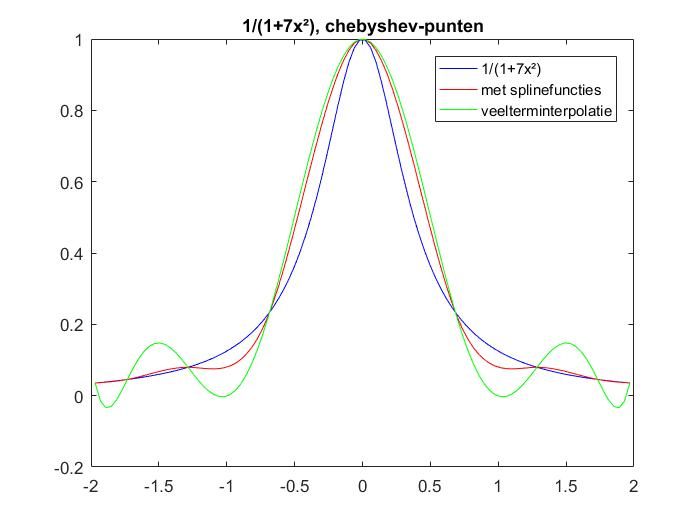
\includegraphics[width=\linewidth]{afbeeldingen/rat_cheb.jpg}
  \caption{functiewaarden}
\end{subfigure}%
\begin{subfigure}{.5\textwidth}
  \centering
  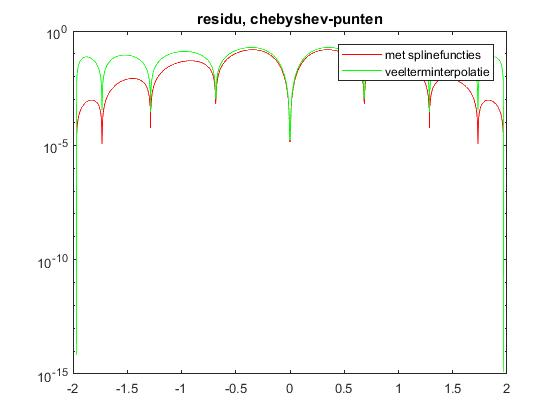
\includegraphics[width=\linewidth]{afbeeldingen/rat_cheb_res.jpg}
  \caption{residu}
\end{subfigure}
\caption{interpolant door 9 Chebychev-punten van  $\frac{1}{1+7x^2}$}
\label{fig:ratcheb}
\end{figure}